\documentclass{beamer}
\newcommand{\q}{\mbox{"}}
\renewcommand{\b}{\mbox{$\tt\backslash$}}
\def\textttb#1{\mcolor{blue}{\texttt{#1}}}
\def\mpause{\pause}
\def\todo#1{\mcolor{red}{\textbf{#1}}}
\usepackage{pgfpages}
%\usepackage{pgfpages}\pgfpagesuselayout{8 on 1}[a4paper,border shrink=1mm, landscape]\def\mpause{}

\usepackage{url}
\usepackage{verbatim}
\usepackage{color}
%\usepackage{bm}
\usepackage{beamerthemesplit}
\defbeamertemplate*{footline}{infolines theme}{
\hspace*{2ex}    \insertframenumber{} / \inserttotalframenumber\hspace*{2ex} 
%   \insertpagenumber{} / \insertpresentationendpage \hspace*{2ex}
  \vskip1ex}

\def\mcolor#1#2{\rule{0ex}{0ex}\color{#1}#2\color{black}{}}
\usetheme{Copenhagen}
%\setbeamercolor{title}{fg=red!80!black,bg=red!20!white}
\makeatletter % code block to allow custom labels to be cross-ref'ed; see comp.text.tex "customized display labels cross-ref'd"
\begin{document}

\title{MSc/ICY Software Workshop\\
Introduction -- Simple Computation, Variables, Types, static Methods}

\author[Manfred~Kerber]{\begin{tabular}{ll}
\mcolor{blue}{Manfred Kerber} &   {\tt www.cs.bham.ac.uk/\~{}mmk}\\
\end{tabular}}

\date{28 September 2016}

\begin{frame}
\titlepage


\end{frame}

\begin{frame}
\frametitle{Overview}

\begin{enumerate}
\item Pocket calculator computations, base types, simple strings, variables, static methods, JavaDoc\\
Fri: 1st Lab Lecture (login, editor, javac, javadoc)

\item Classes, objects, methods, JUnit tests\\
Fri: 2nd Lab Lecture (Eclipse)

\item Conditionals, `for' Loops, arrays, ArrayList\\

\item Exceptions, assertions, I/O, Patterns, printf

\item Interfaces, functions

\item Sub-classes, inheritance, abstract classes

\item Inheritance (Cont'd), packages

\item Graphics

\item Graphical User Interfaces

\item Graphical User Interfaces (Cont'd)

\item Revision
\end{enumerate}
Changes possible
\end{frame}

\begin{frame}
\frametitle{Structure}
\begin{itemize}
\item \mcolor{blue}{Lectures:}
   \begin{itemize}
     \item Wednesdays 10:00-12:00, 203 Haworth
     \item planned Fridays 9:00-11:00 \mcolor{red}{UG Lab Computer Science}\\
          \hspace*{3ex}Weeks 6 \& 10 (4 Nov \& 2 Dec), Aston Webb C, Main LT
   \end{itemize}

\item\rule{0ex}{4ex} \mcolor{blue}{Tutorials:}
   \begin{itemize}
     \item Tuesdays, 1 hour, see separate sheet.\\
       \mcolor{red}{Attendance to the tutorials is compulsory.}
     \item Different groups streamed according to background knowledge
       and self-assessment.

   \end{itemize}
\item\rule{0ex}{4ex} \mcolor{blue}{Labs:}
   \begin{itemize}
     \item Mondays 13:00-15:00
     \item Thursdays 11:00-14:00
   \end{itemize}
\end{itemize}
\end{frame}

\begin{frame}
\frametitle{Assessment}
This module is a 40cr module over two terms. $\sim$50\% of the module mark are on the 20cr of this term. \bigskip

\mcolor{blue}{The overall mark is computed as:}
\begin{itemize}
\item  70\% Examination in May/June 2017
\item  20\% Continuous Assessment Term 1 and Term 2
\item  10\% Team Project in Term 2
\end{itemize}

This term the Continuous Assessment is partly in form of Worksheets
which must be submitted via Canvas, and partly in form of In-Class
tests.

MSc students need an overall mark of at least 50, ICY students an
overall mark of at least 40 in order to pass this module.
\end{frame}

\begin{frame}
\frametitle{Continuous Assessment}
\begin{tabular}{|l@{\quad}|r@{\quad}|r@{\ }r@{\qquad}|r|c|}\hline
Assignment&Hand out&&Hand in &  \%  & Marking\\\hline\hline
 WS 1   &  Wk1 & Wk2& 6 Oct  &  0   & - \\\hline %%% unassessed
 WS 2   &  Wk2 & Wk4&20 Oct  &  9   & Tests\\\hline
        &  Wk3 &    &        &      & \\\hline
 WS 3   &  Wk4 & Wk6&3 Nov   &  9   & Tests\\\hline
        &  Wk5 &    &        &      & \\\hline
 WS 4   &  Wk6 & Wk8&17 Nov  &  9   & Tests\\
 Test 1 &(4 Nov)&Wk6& (4 Nov)&  9   & Paper\\\hline
        &  Wk7 &    &        &      & \\\hline
 WS 5   &  Wk8 &Wk10& 1 Dec  &  9   & Viva \\\hline
        &  Wk9 &    &        &      & \\\hline
 WS 6   &  Wk10&WkS1& 9 Jan  &  9   & Viva\\
 Test 2 &(2 Dec)&Wk10&(2 Dec)&9     & Paper\\\hline
        & Wk11      &  &     &      & \\\hline

\end{tabular}\smallskip

\mcolor{blue}{[Changes possible but not planned]}. All Worksheet
hand-ins are at 2pm sharp. Late submission invokes a penalty of 5
marks. No hand-in after 24 hours.

\end{frame}

\begin{frame}
\frametitle{Plagiarism}
\begin{itemize}
\item You can and are advised to cooperate in your revision, in the Friday lab lectures, and in understanding the exercises.
\item You \mcolor{red}{must not collaborate} in writing the code for the Worksheets and also \mcolor{red}{must not cheat} in the two in-class tests.
\item The University's Code of Practice on plagiarism is at {\footnotesize\url{www.birmingham.ac.uk/Documents/university/legal/plagiarism.pdf}}, and\\ the School guidance notes are at
\url{http://www.cs.bham.ac.uk/internal/taught-students/plagiarism}
\end{itemize}
\end{frame}



\begin{frame}
\frametitle{Reading} 
In order for the lectures being most effective you are expected
to have read the corresponding material \mcolor{red}{BEFORE} the lectures!\bigskip

\begin{minipage}{0.50\textwidth}
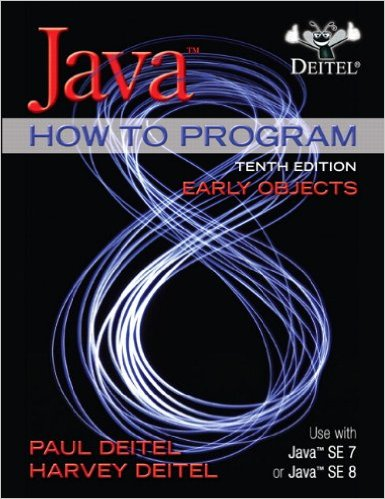
\includegraphics[height=5cm]{deitel10} 
\end{minipage}
\begin{minipage}{0.45\textwidth}
{\Large Paul \mcolor{blue}{Deitel},\\ Harvey \mcolor{blue}{Deitel}\\
 Java - How to Program\\
Tenth Edition}

\mcolor{blue}{Week 1: Chapters 1 \& 2}\\
\mcolor{blue}{Week 2: Chapter 3}
\end{minipage}\bigskip

{\small [Note: There are other books which cover the same material. You are
free to choose a different book for your reading. However, I will
indicate the reading according to the book above.]}
\end{frame}

\begin{frame}
\frametitle{The Java programming language}
\Large
Java is
\begin{itemize}
  \item platform independent
  \item object-oriented
  \item strictly typed
\end{itemize}\bigskip

We will learn in more depth what this means in the course of the next
few weeks.
\end{frame}

\begin{frame}
\frametitle{A simple program}

In a few simple steps to a \texttt{HelloWorld} program:

\begin{enumerate}
 \item Open a file \textttb{HelloWorld.java} in an editor like \texttt{jedit} or \texttt{gedit}
 \item Write the program starting with\\
      \textttb{public class HelloWorld}\\
      Note that the name of the class here must match the filename.
 \item Save the file.
 \item Compile the program on the command line by\\
      \textttb{javac HelloWorld.java}\\
  This generates a file \textttb{HelloWorld.class}.
 \item Run the program on the command line by\\
      \textttb{java HelloWorld}
 \item Extract documentation on the command line by\\
      \textttb{javadoc HelloWorld.java}
\end{enumerate}
\end{frame}

\begin{frame}
\frametitle{The full HelloWorld program}
\verbatiminput{HelloWorld.java}
\end{frame}

\begin{frame}
\frametitle{Comments}
\begin{itemize}
\item Java is to be understood by \mcolor{blue}{computers}
  \mcolor{red}{and} \mcolor{blue}{humans}.

\item \mcolor{blue}{Computers} translate programs into a level (by an
  interpreter or by a compiler) that can be executed command by
  command in the order given by the programmer.

\item \mcolor{blue}{Humans} translate programs into something that is meaningful to them.

\item If somebody reads somebody else's code (or even their own code
  after a while) then they may have problems to understand it. 
  What is done in the program? Why is it done? How is it done?
  When will it work and when not? Does it come with a Best-Before date?
  Who owns the copyright? Where may it be applied and where not?
  All relevant information should be written in the program as \mcolor{blue}{comments}.

\item  In Java, everything between /* and */ is a comment.

\item Everything between an opening /** and */ is considered by
  JavaDoc.
\end{itemize}
\end{frame}

\begin{frame}
\frametitle{Strings}
\begin{itemize}
\item If a String contains \texttt{\q} then it is represented by \texttt{$\tt\b$\q}.
\item Strings can be put together (concatenated) by \texttt{+}.\\ E.g.\
  \texttt{\q{}Hello\q{} + \q{}World\q{}} is the string \texttt{\q{}HelloWorld\q{}}.
\item We can print Strings by something like \mcolor{blue}{\texttt{System.out.println(\q{}Hello World\q{});}}
\end{itemize}
\end{frame}

\begin{frame}
\frametitle{Variables}
\begin{itemize}
\item All variables must be \mcolor{blue}{declared} with a type such as\\ \textttb{public int x;}.
\item It is possible to declare several variables of the same type in a single step \textttb{public int x, y, z, u, v;}
\item Before a variable is used it must be \mcolor{blue}{initialized}, that is, it must be given an initial value.
  E.g., by the assignment \textttb{x = 3;}. The value can be
  overwritten by a new assignment, e.g., by writing after the first assignment a second such as \textttb{x = 4;}.\\
(In such a case the previous value is irrecoverably gone.)
\end{itemize}
\end{frame}

\begin{frame}
\frametitle{Variables (Cont'd)}
Think of variables as names plus their values, represented in a
table as follows:
\mcolor{red}{\begin{center}
\begin{tabular}{|l||c|c|c|c|c|}\hline
	  name &  x  &  y  &  z  &  u  &  v \\\hline
	  val  &  -  &  -  &  -  &  -  &  - \\\hline
\end{tabular}
\end{center}}

After an assignment \textttb{var = term;} the term on the right hand side is
evaluated with respect to the current values in the table.

The assignment \textttb{x = 3;} means that the table is updated, any
old value of \textttb{x} (or no value in this case) is overwritten by
the new value. If the old value is
still needed, it must be copied before the assignment,
since after the assignment the value is lost.
\mcolor{red}{\begin{center}
\begin{tabular}{|l||c|c|c|c|c|}\hline
	  name &  x  &  y  &  z  &  u  &  v \\\hline
	  val  &  3  &  -  &  -  &  -  &  - \\\hline
\end{tabular}
\end{center}}
\end{frame}

\begin{frame}
\frametitle{Variables (Cont'd)}
\vspace*{-2ex}\mcolor{red}{\begin{center}
\begin{tabular}{|l||c|c|c|c|c|}\hline
	  name &  x  &  y  &  z  &  u  &  v \\\hline
	  val  &  3  &  -  &  -  &  -  &  - \\\hline
\end{tabular}
\end{center}}

After the assignment \textttb{y = 2*(x+5);} the table is computed by
evaluating the expression \textttb{2*(x+5)} in the OLD TABLE and then
overwriting the current value of y by the result.\mpause
\vspace*{-1ex}\mcolor{red}{\begin{center}
\begin{tabular}{|l||c|c|c|c|c|}\hline
	  name &  x  &  y  &  z  &  u  &  v \\\hline
	  val  &  3  &  16  &  -  &  -  &  - \\\hline
\end{tabular}
\end{center}}\mpause

After the assignment \textttb{y = 2*(y+x*x);}\mpause
\vspace*{-1ex}\mcolor{red}{\begin{center}
\begin{tabular}{|l||c|c|c|c|c|}\hline
	  name &  x  &  y  &  z  &  u  &  v \\\hline
	  val  &  3  &  50  &  -  &  -  &  - \\\hline
\end{tabular}
\end{center}}\mpause

After the assignments \textttb{z = x+y; u = 3*z; x = 0;}
the table is:\mpause
\vspace*{-1ex}\mcolor{red}{\begin{center}
\begin{tabular}{|l||c|c|c|c|c|}\hline
	  name &  x  &  y  &  z  &  u  &  v \\\hline
	  val  &  0  &  50  &  53  &  159  &  - \\\hline
\end{tabular}
\end{center}}
\end{frame}

\begin{frame}
\frametitle{Variables (Cont'd)}
\mcolor{red}{\begin{center}
\begin{tabular}{|l||c|c|c|c|c|}\hline
	  name &  x  &  y  &  z  &  u  &  v \\\hline
	  val  &  0  &  50  &  53  &  159  &  - \\\hline
\end{tabular}
\end{center}}

If variables are needed for this evaluation which do not have a value
yet -- indicated by the hyphen in the table -- then the assignment
fails and an error occurs. E.g. \textttb{v = v+1;} would fail since
\textttb{v} has currently no value. However, \textttb{x = x+1;}
succeeds since the expression on the right hand can be evaluated.
\end{frame}

\begin{frame}
  \frametitle{Types} 
  Java has 8 different \mcolor{blue}{base types}, 4 for the
  representation of integers, 2 for floating point numbers, 1 for
  boolean values, and 1 for characters.\mpause

Integers are implemented in a cyclic way (such as a clock):\mpause

\begin{tabular}{ll}
  \mcolor{blue}{byte}  & range -128 to 127\\

  \mcolor{blue}{short} & range -32,768 to 32,767\\

  \textbf{\mcolor{red}{int}}   & range -2,147,483,648 to  2,147,483,647\\

  \mcolor{blue}{long}  & range -9,223,372,036,854,775,808 to\\
             & \phantom{range -}9,223,372,036,854,775,807
\end{tabular}

Floating point numbers (reals) are approximated by 4 or 8 bytes

\begin{tabular}{ll}
  \mcolor{blue}{float} & 4 bytes, 6-7 significant decimal digits\\
        &  3.4028235E38\\
  \textbf{\mcolor{red}{double}} & 8 bytes
\end{tabular}

The type \mcolor{blue}{booleans} contains two elements:
\texttt{true} and \texttt{false}.

The type \mcolor{blue}{char} is used to represent characters such as
\texttt{'a'}, \texttt{'b'}, \texttt{'c'}, and
\texttt{'$\backslash$u00A3}' (for the pound symbol). They are enclosed
in single quotes.

\end{frame}

\begin{frame}
\frametitle{Methods}
Assume the computation of the areas of squares:
\begin{itemize}
\item $\tt 7.932 * 7.932$
\item $\tt 8.2   * 8.2$
\item $\tt 13.87 * 13.87$
\item $\tt 123.89 * 123.89$
\end{itemize}

In order to avoid the repetition of the values we would like to write a method that computes the values as
\begin{itemize}
\item $\tt square(7.932)$
\item $\tt square(8.2)$
\item $\tt square(13.87)$
\item $\tt square(123.89)$
\end{itemize}
\end{frame}

\begin{frame}
\frametitle{Methods (Cont'd)}
\verbatiminput{Square.java}

\begin{itemize}
\item \texttt{public} means that the method can be called by anybody who can access the class. 
\item \texttt{static} we ignore for now.
\item the first \texttt{int} is the return type.
\item \texttt{square} is the name of the method with which it is ``called.''
\item the second \texttt{int} is the type of the parameter \texttt{x}.
\item \texttt{x} is the name of the parameter.
\item \texttt{return} specifies what the method gives back as value.
\end{itemize}

This method is called by something like \texttt{square(4)}.
\end{frame}

\begin{frame}
\frametitle{What Next?}

\begin{enumerate}
 \item \mcolor{red}{Lab lecture} UG lab CS on Friday
%    \begin{description}
%      \item[9--10 am] Surname starting with A--L
%      \item[10--11 am] Surname starting with M--Z
%    \end{description}
  \item Follow the pages on\\ 
        \url{https://birmingham.instructure.com/courses/21955}

  \item Discussions possible on\\
        \url{https://www.facebook.com/groups/346033342153057/}

  \item \mcolor{blue}{More Examples}
\end{enumerate}
\end{frame}
\end{document}
